\documentclass[a4paper]{report}
\usepackage[utf8]{inputenc}
\usepackage[portuguese]{babel}
\usepackage{hyperref}
\usepackage{a4wide}
\hypersetup{pdftitle={VC - Turorial 2},
pdfauthor={José Ferreira, Luís Pereira},
colorlinks=true,
urlcolor=blue,
linkcolor=black}
\usepackage{subcaption}
\usepackage{listings}
\usepackage{booktabs}
\usepackage{multirow}
\usepackage{appendix}
\usepackage{tikz}
\usepackage{authblk}
\usepackage{bashful}
\usepackage{verbatim}
\usepackage{amssymb}
\usepackage{multirow}
\usepackage{mwe}
\usepackage{float}
\usetikzlibrary{positioning,automata,decorations.markings}

\begin{document}

\title{VC - Tutorial 2}
\author{José Ferreira (A83683), Luís Ferreira (A86265)}
\date{\today}

\begin{center}
    \begin{minipage}{0.75\linewidth}
        \centering
        
\includegraphics[width=0.4\textwidth]{images/eng.jpeg}\par\vspace{1cm}
        \vspace{1.5cm}
        \href{https://www.uminho.pt/PT}
        {\color{black}{\scshape\LARGE Universidade do Minho}} \par
        \vspace{1cm}
        \href{https://www.di.uminho.pt/}
        {\color{black}{\scshape\Large Departamento de Informática}} \par
        \vspace{1.5cm}
        \maketitle
    \end{minipage}
\end{center}

\tableofcontents

\pagebreak
\chapter{Introdução}
No âmbito da Unidade Curricular de Visão por Computador, foi-nos proposto
criar um programa em \textit{Matlab} com a funcionalidade de retirar
informação sobre a localização dos pés de uma dada imagem. Esta tanto
pode ser uma imagem \textit{RGB} ou uma imagem de profundidade. Para apresentar estes
resultados,as coordenadas são indicadas através das
coordenadas da ponta do pé e as coordenadas do calcanhar.

Para além de ser capaz de identificar estas coordenadas numa imagem, o programa
também deve ser capaz de detetar estas coordenadas num vídeo.

Ao longo deste relatório iremos descrever os passos tomados para realizar este
programa. Primeiramente, iremos descrever como fizemos a detecção das
coordenadas numa imagem e aprimoramos o resultado. Em seguida iremos explicar
como foi feita a adaptação para funcionar com um vídeo. Finalmente, iremos
apresentar o resultado final.

\chapter{Deteção de pés numa imagem}
Ao longo deste capítulo iremos descrever a metodologia usada para detetar as
coordenadas da ponta dos pés e do calcanhar.

Para a realização deste objetivos temos acesso a dois tipos distintos de dados.
Temos acesso a uma câmera \textit{RGB} e acesso a uma câmera de profundidade. A estratégia
escolhida envolve usar os dados contidos na câmera de profundidade, sendo que a
imagem capturada pela câmera \textit{RGB} é apenas usada para mostrar o resultado de uma
forma visual e apelativa.

\begin{figure}[H]
\centering
\begin{minipage}{.5\textwidth}
  \centering
    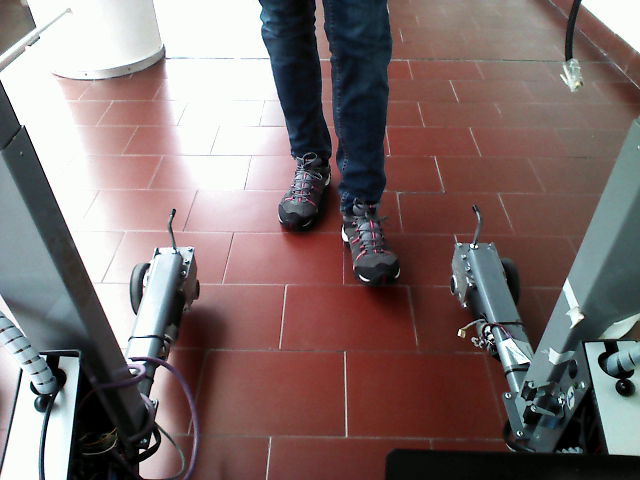
\includegraphics[width=0.99\textwidth]{images/og/gait_RGB_oneimage.png}
    \captionof{figure}{Imagem RGB}
\end{minipage}%
\begin{minipage}{.5\textwidth}
  \centering
    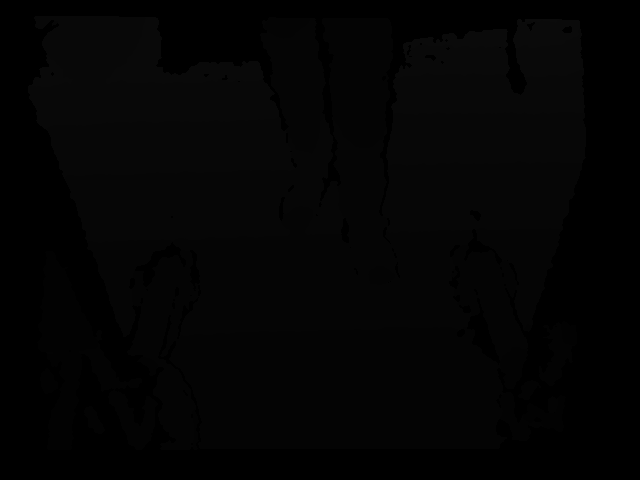
\includegraphics[width=0.99\textwidth]{images/og/gait_depth_oneimage.png}
    \captionof{figure}{Imagem de profundidade}
\end{minipage}%
\end{figure}

\section{Área de Interesse}
Primeiramente, definimos uma área de interesse no ecrã, para ser mais fácil processar
os dados. Desta forma temos de processar uma menor quantidade de pixeis e evitamos
erros que podem, eventualmente, ser introduzidos por objetos, como as pernas do
andarilho.

A princípio, a área que definimos era um losango, para se adaptar à perspectiva da
câmera, mas após termos realizado várias experiências, chegamos à conclusão que um
retângulo cobriria a mesma área, com a mesma eficiência. Para além disso, o
desenvolvimento do programa torna-se muito mais fácil devido a uma maior
simplicidade matemática.

Na imagem abaixo está representada a área de interesse através da sobreposição
de um retângulo vermelho sobre a imagem \textit{RGB} original.

\begin{figure}[H]
    \centering
        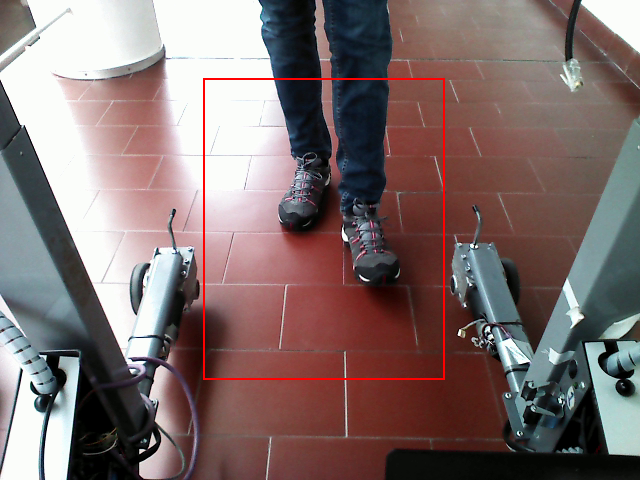
\includegraphics[width=0.6\textwidth]{images/building/area_of_interest.png}
        \caption{Área de interesse (vermelho)}
\end{figure}


\vspace{1cm}

\section{Thresholding}
Munidos agora da área, onde apenas se encontram os pés, as pernas e o
chão, temos de alguma forma eliminar os restantes elementos para ficar apenas com
os pés.

Os pés encontram-se numa faixa de altura ao chão, sendo que acima disso temos as
pernas e abaixo temos o chão. Isto representa um problema de \textit{threshold}.
O problema é que a distância, ou seja, o \textit{threshold}, tem de variar ao longo da imagem,
porque existe perspectiva, ou seja, a câmera encontra-se a um certo ângulo do chão. Por exemplo,
o chão que se encontra mais abaixo na imagem está mais perto da câmera, enquanto que o que se
encontra mais acima, já se encontra a um maior nível de profundidade.

De modo a calcular este \textit{threshold}, pensamos em utilizar o ângulo da câmera e a altura
desta ao solo. No entanto, se este valor não for medido de forma precisa o resultado
final perderia qualidade. Para além disto, qualquer alteração na posição da câmera, para,
por exemplo, acomodar uma pessoa maior, implicaria alterar parâmetros no software.

Por isto, decidimos criar uma solução que não envolvesse valores para além dos fornecidos
pela câmera de profundidade. 

Após analisar o problema, chegamos à conclusão que para uma
dada linha da área de interesse existem duas propriedades que se mostram verdadeiras:
o chão encontra-se à mesma distância ao longo desta linha e a distância máxima registada
nessa linha tem de ser o chão.

Assim, se pegarmos no maior valor de cada linha da área de interesse, obtemos uma
aproximação da distância ao chão nessa dada linha. Escolhemos, então, dois valores de
\textit{threshold} (que serão futuramente otimizados), de forma a tentar isolar ao máximo
os pés, tendo estes sido pintados de preto e tudo o resto de branco, criando uma imagem binarizada,
sendo que a Figura \ref{img:simple_max_feet} pretende apresentar apenas os pés. 


\begin{figure}[H]
\centering
\begin{minipage}{.5\textwidth}
  \centering
    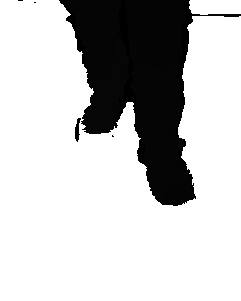
\includegraphics[width=0.85\textwidth]{images/building/max_legs.png}
    \captionof{figure}{Eliminar chão}
    \label{img:simple_max_legs}
\end{minipage}%
\begin{minipage}{.5\textwidth}
  \centering
    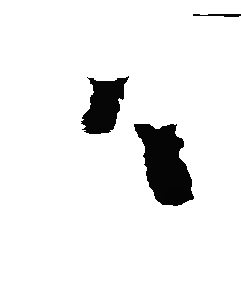
\includegraphics[width=0.85\textwidth]{images/building/max_feet.png}
    \captionof{figure}{Capturar pés}
    \label{img:simple_max_feet}
\end{minipage}%
\end{figure}

Como se pode observar, ainda existe algum ruído presente. Este ruído pode advir do
facto de existirem erros na medição da câmera, fazendo com que o valor máximo numa
linha não seja o do chão.

Para além disso, grande parte da ponta do pé ficou cortada, porque de forma a reduzir
o ruído, o \textit{threshold} teve de ser aumentado, acabando por intercetar com os valores correspondentes ao pé.

Para remediar estes dois problemas, decidimos criar uma função semelhante à \texttt{max}, mas
que em vez de devolver o máximo de cada linha, devolve a média dos N maiores valores de cada
linha. Desta forma podemos eliminar valores extremos nas linhas e diminuir o \textit{threshold}
sem aumentar o ruído, de forma a capturar mais do pé.

\begin{figure}[H]
\centering
\begin{minipage}{.5\textwidth}
  \centering
    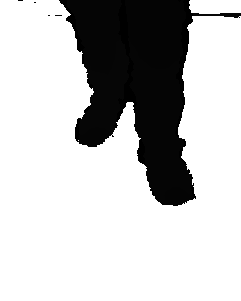
\includegraphics[width=0.85\textwidth]{images/building/special_max_legs.png}
    \captionof{figure}{Eliminar chão}
\end{minipage}%
\begin{minipage}{.5\textwidth}
  \centering
    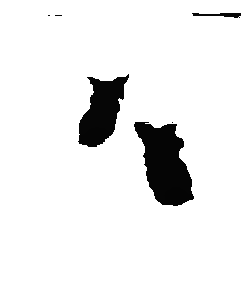
\includegraphics[width=0.85\textwidth]{images/building/special_max_feet.png}
    \captionof{figure}{capturar pés}
\end{minipage}%
\end{figure}

Finalmente, tendo em conta que o chão é plano na área que estamos a tratar, podemos
obter a função que melhor se adapta aos valores calculados para cada linha, fazendo
uso da função \texttt{polyfit} definida em \texttt{Matlab}. Com recurso a essa função podemos criar
os valores, eliminando ainda mais possíveis erros. Desta forma podemos aumentar mais o
\textit{threshold} e eliminar completamente o ruído presente anteriormente, mantendo a qualidade
da área do pé detetada.

\begin{figure}[H]
\centering
\begin{minipage}{.5\textwidth}
  \centering
    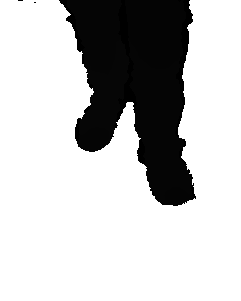
\includegraphics[width=0.85\textwidth]{images/building/compensated_max_legs.png}
    \captionof{figure}{Eliminar chão}
\end{minipage}%
\begin{minipage}{.5\textwidth}
  \centering
    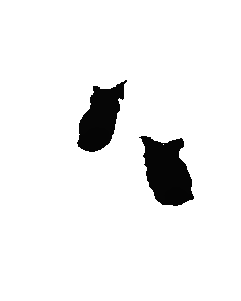
\includegraphics[width=0.85\textwidth]{images/building/compensated_max_feet.png}
    \captionof{figure}{Capturar pés}
\end{minipage}%
\end{figure}

\section{Close e Dilate}
Após o processo de \textit{thresholding}, ainda é possível encontrar algum ruído nas imagens geradas.
Isto pode ser criado por algum desbalanceamento no chão ou até mesmo ruído próprio da imagem de
profundidade. O \textit{frame} que encontramos mais atingido por este problema é o número 00.

\begin{figure}[H]
    \centering
        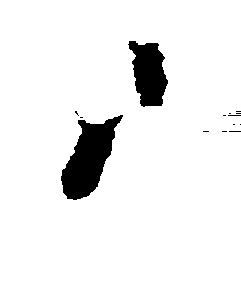
\includegraphics[width=0.4\textwidth]{images/building/closeDilate/original00.png}
        \caption{Frame de profundidade 00}
        \label{img:frame00}
\end{figure}

Como se pode observar, no lado direito da imagem, algumas linhas ficaram com pixeis indesejados pintados
a preto. Ao mesmo tempo, também é de reparar que o formato do pé obtido não é dos mais fáceis de trabalhar
para encontrar o dedo e calcanhar do pé. O pretendido seria mais um losango ou retângulo, ou seja, com o
menor relevo possível, algo que tanto os cordões como algum ruído foi criado na imagem.

Com o objetivo de eliminar estes dois problemas foi escolhido o uso de operações morfológicas binárias. A
operação conhecida por remover o ruído preto é a chamada de \texttt{closing}. Esta é composta pela
combinação de uma \texttt{dilation} seguida de uma \texttt{erosion}. O nome destas operações é contra-intuitivo
no ambiente em que nos encontramos, pois temos pés pretos com \textit{background} branco e apenas seria
observada dilatação e erosão dos pés se estes fossem brancos e o \textit{background} preto. 

A \texttt{dilation} vai, então, usar um \textit{kernel} com formato e tamanho pré-definidos, de modo a
que cada pixel preto que esteja a ser processado, se algum dos pixeis que estão dentro do \textit{kernel}
seja branco, este pixel a ser processado também passa para branco.

No nosso caso, o valor de \textit{kernel} que originou no resultado melhor foi um quadrado com um
tamanho de 13, que sendo aplicado na Figura \ref{img:frame00} resulta na seguinte figura.

\begin{figure}[H]
    \centering
        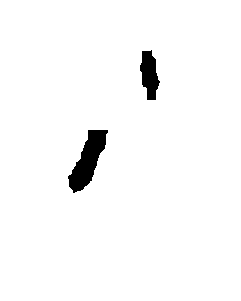
\includegraphics[width=0.4\textwidth]{images/building/closeDilate/dilate13.png}
        \caption{Frame após dilation}
        \label{img:dilation13}
\end{figure}

Com esta imagem é verificado que o ruído encontrado na imagem inicial foi removido, tanto o dos
cordões do sapato, como o encontrado no lado direito da imagem.

De seguida, com o objetivo de retornar os pés ao seu tamanho original, mas com o ruído tratado e com
a remoção dos cordões é necessário realizar a operação \textit{erosion} com o mesmo \textit{kernel},
de forma a finalizar a operação \texttt{close}.

A \texttt{erosion}, semelhantemente à operação anterior, vai usar um \textit{kernel} com formato e
tamanho pré-definidos. Desta vez, cada pixel branco que esteja a ser processado, se algum dos outros
pixeis, que se encontram dentro do \textit{kernel}, seja preto, o pixel a ser processado também passa
para preto.

Executando esta operação ao resultado visualizado na Figura \ref{img:dilation13}, com o mesmo
\textit{kernel} da operação anterior, é possível obter, então, o resultado da operação morfológica
\texttt{close} que é gerado na seguinte imagem.

\begin{figure}[H]
    \centering
        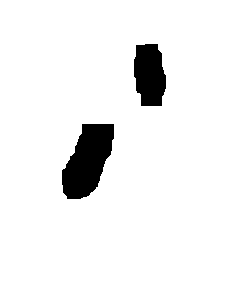
\includegraphics[width=0.4\textwidth]{images/building/closeDilate/erode13.png}
        \caption{Frame após erosion}
        \label{img:erode13}
\end{figure}

É conseguido assim ter uma imagem dos pés sem ruído e com um formato mais satisfatório.

De notar que se fosse aplicado um \textit{kernel} com diferente formato ou com tamanho diferentes
os resultados não seriam os mais desejados, como se pode observar nas seguintes imagens.


\begin{figure}[H]
\centering
\begin{minipage}{.5\textwidth}
  \centering
    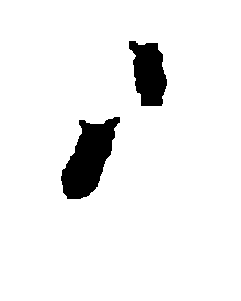
\includegraphics[width=0.52\textwidth]{images/building/closeDilate/close5.png}
    \captionof{figure}{Close com kernel = 5}
\end{minipage}%
\begin{minipage}{.5\textwidth}
  \centering
    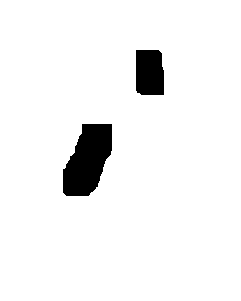
\includegraphics[width=0.52\textwidth]{images/building/closeDilate/close23.png}
    \captionof{figure}{Close com kernel = 23}
\end{minipage}%
\end{figure}
\begin{figure}[H]
\centering
\begin{minipage}{.5\textwidth}
  \centering
    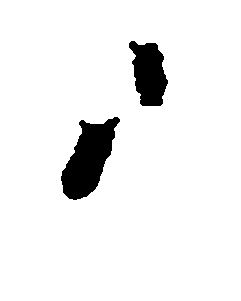
\includegraphics[width=0.52\textwidth]{images/building/closeDilate/disk.png}
    \captionof{figure}{Close com kernel em disco}
\end{minipage}%
\begin{minipage}{.5\textwidth}
  \centering
    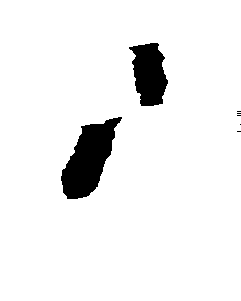
\includegraphics[width=0.52\textwidth]{images/building/closeDilate/line.png}
    \captionof{figure}{Close com kernel em linha}
\end{minipage}%
\end{figure}

Por fim, de modo a preparar para a obtenção das coordenadas do dedo do pé prentendido e do
calcanhar é necessário ter o verdadeiro tamanho pé, pois o que temos é o tamanho aproximado
do sapato. Para atingir isso é necessário realizar uma erosão no sapato, que como mencionado
anteriormente, ao ser contra-intuitivo é obtido através de um \textit{dilate}. O kernel escolhido
foi um de tamanho 9 e, mais uma vez, formato quadrado, que aplicado à Figura \ref{img:erode13}
surgindo a seguinte imagem.

\begin{figure}[H]
    \centering
        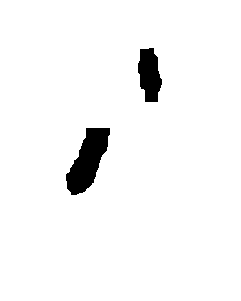
\includegraphics[width=0.4\textwidth]{images/building/closeDilate/finalOperation.png}
        \caption{Frame após dilatação}
        \label{img:finalOperation}
\end{figure}

Observa-se, assim, a desejada diminuição da região preta, tornando a imagem pronta para o algoritmo
de obtenção das coordenadas pretendidas.

\section{Obtenção das coordenadas}
Para a obtenção das coordenadas foi desenvolvido um algoritmo com o intuito de ultrapassar todos os
obstáculos encontrados.

O primeiro encontra-se na dificuldade de descobrir a região que corresponde ao pé direito e ao esquerdo.

\begin{figure}[H]
    \centering
        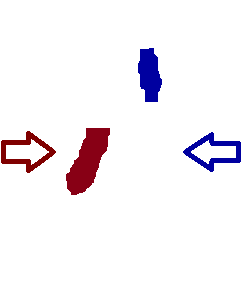
\includegraphics[width=0.3\textwidth]{images/building/coords/finalOperationColor.png}
        \caption{Frame colorido}
        \label{img:finalOperationColor}
\end{figure}

 A solução selecionada correspondeu a percorrer primeiro as colunas da esquerda para a direita para
 encontrar o pé direito (pintado a vermelho) e de seguida da direita para a esquerda para encontrar
 o pé esquerdo (pintado a azul).
 
 Ao ser encontrado o ponto mais à esquerda do pé direito (vermelho) são avançadas 5 colunas para a
 direita e vai se descendo até encontrar a fronteira do pé. É assim selecionado o ponto correspondente
 ao dedo do pé direito. De maneira semelhante é encontrado o dedo no pé esquerdo (azul), com a nuance
 de que após ser encontrado o ponto mais à direita são deslocadas 5 colunas para a esquerda para de seguida
 descer.
 
 Voltando à primeira coluna onde foi encontrado o pé direito, é então retomada a iteração através das
 colunas, desta feita até encontrar a primeira coluna que tem todos os seus pixeis de cor branca. Assim
 que esta for descoberta são recuadas 6 colunas e selecionado o ponto preto mais a norte. Para o pé
 esquerdo é realizado o processo equivalente.
 
 O resultado de todo este processo pode ser visualizado na seguinte imagem, onde os pontos selecionados
 estão unidos por uma linha, em ambos os pés.


\begin{figure}[H]
    \centering
        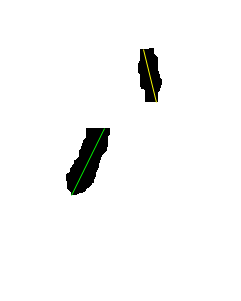
\includegraphics[width=0.4\textwidth]{images/building/coords/coordsInitial.png}
        \caption{Frame com os pontos selecionados}
\end{figure}

Pode também ser visualizado como o resultado fica na imagem após \textit{thresholding}, assim como na área de interesse na imagem \textit{RGB}.

\begin{figure}[H]
\centering
\begin{minipage}{.5\textwidth}
  \centering
    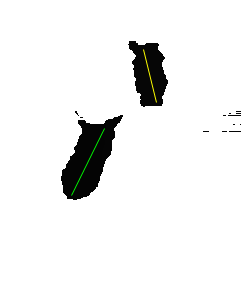
\includegraphics[width=0.61\textwidth]{images/building/coords/coordsOriginal.png}
    \captionof{figure}{Antes das operações morfológicas}
\end{minipage}%
\begin{minipage}{.5\textwidth}
  \centering
    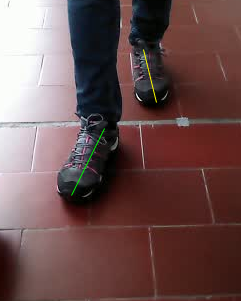
\includegraphics[width=0.61\textwidth]{images/building/coords/coordsRGB.png}
    \captionof{figure}{Área de interesse RGB}
\end{minipage}%
\end{figure}

\chapter{Deteção de pés num vídeo}
Para além de receber apenas uma imagem de teste, também recebemos uma pasta com as imagens que
correspondem às imagens de profundidade de um dado vídeo. Para analisar estas imagens decidimos
criar uma função que utiliza a função definida no capítulo anterior. Esta função aplica para 
todas as imagens dentro da pasta a função que devolve as coordenadas dos pés
e guarda as imagens com os diagramas indicativos do resultado numa outra pasta (output). Para permitir este
\textit{debug} também precisa de receber um vídeo \textit{RGB} a que as imagens de profundidade
correspondem.

\chapter{Análise de Resultados}

Para proceder a uma análise dos resultados, inicialmente, escrevemos os dados obtidos para
uma folha de cálculo com o mesmo formato dos valores de \textit{ground truth} fornecidos.

Apesar dos nossos resultados estarem visualmente próximos do pretendido, os valores eram
bastante diferentes dos fornecidos.

Com o objetivo de comparar os resultados, colocamos os mesmos \textit{frames} lado a lado, com o \textit{ground
truth} à esquerda e os nossos \textit{frames} do lado direito. Comparando os resultados obtidos os
nossos aparentam estar mais próximos em quase todos os casos da realidade do que o \textit{ground truth}.

Analisando, mais a fundo, seis \texttt{frames} espaçados no tempo uniformemente, ou seja, os  \texttt{frames 00, 10, 20, 30, 40, 50 e 59}, existem casos em que os resultados do \textit{ground truth} estão
bastante longe dos esperados e considerados corretos pelo grupo, nomeadamente no
\texttt{Frame20} e \texttt{Frame30}, representados pelas Figuras \ref{img:Frame20} e
\ref{img:Frame30}.
Por outro lado, os resultados obtidos pelo nosso programa são menos precisos quando
o pé está levantado na parte de trás, este poderia ser atenuado ajustado os valores de threshold, mas em contrapartida haveria um agravamento do valor do calcanhar nos outros \textit{frames}, onde estes apareceriam mais atrás. Como referência temos o \texttt{Frame10} e o
\texttt{Frame59}, reproduzidos nas Figuras \ref{img:Frame10} e \ref{img:Frame59}.

Para além das seguintes imagens enviamos também em anexo um \textit{gif} que representa todas as imagens
obtidas em sequência animadas.

\begin{figure}[H]
\centering
\begin{minipage}{.5\textwidth}
  \centering
    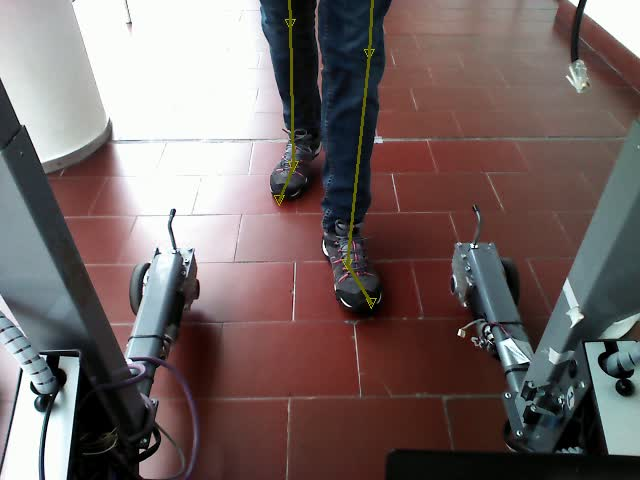
\includegraphics[width=0.98\textwidth]{images/building/results/frameGT00.png}
    \captionof{figure}{Frame 00 Ground Truth}
\end{minipage}%
\begin{minipage}{.5\textwidth}
  \centering
    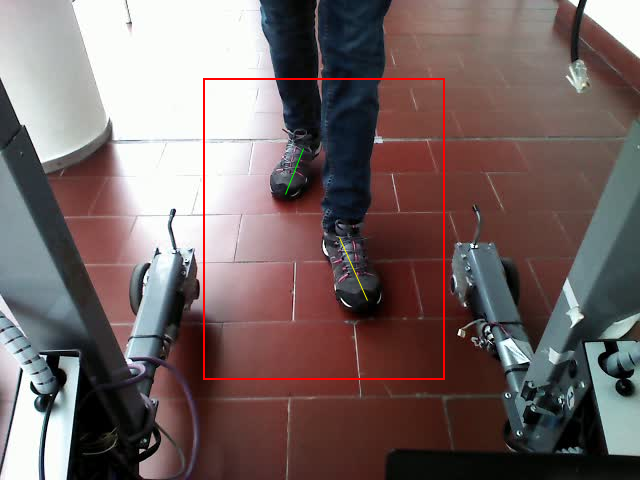
\includegraphics[width=0.98\textwidth]{images/building/results/frame00.png}
    \captionof{figure}{Nosso Frame 00}
    \label{img:Frame00}
\end{minipage}%
\end{figure}

% \begin{figure}[H]
% \centering
% \begin{minipage}{.5\textwidth}
%   \centering
%     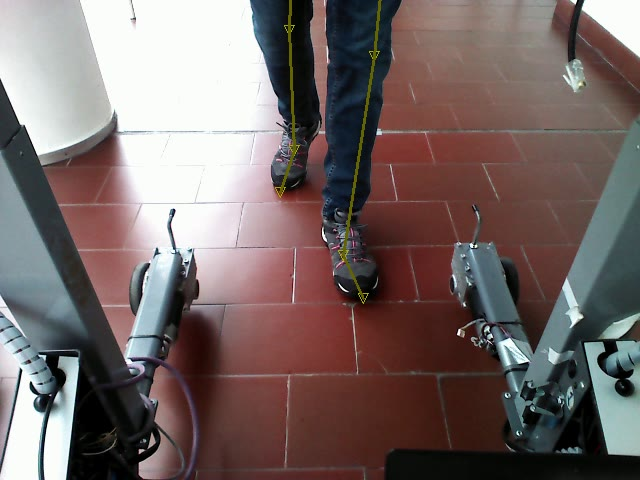
\includegraphics[width=0.98\textwidth]{images/building/results/frameGT05.png}
%     \captionof{figure}{Frame 05 Ground Truth}
% \end{minipage}%
% \begin{minipage}{.5\textwidth}
%   \centering
%     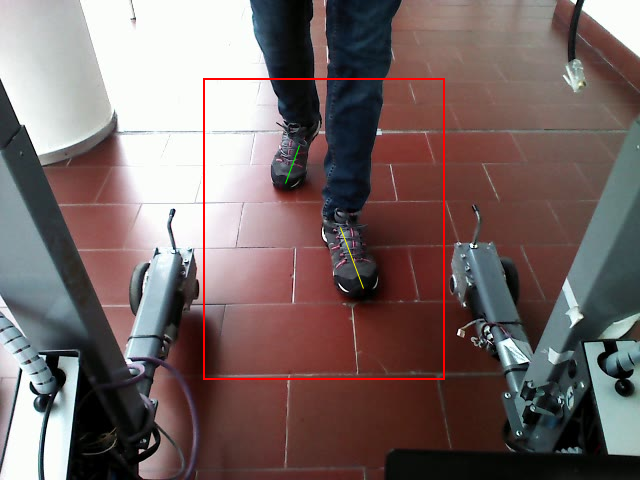
\includegraphics[width=0.98\textwidth]{images/building/results/frame05.png}
%     \captionof{figure}{Nosso Frame 05}
% \end{minipage}%
% \end{figure}

\begin{figure}[H]
\centering
\begin{minipage}{.5\textwidth}
  \centering
    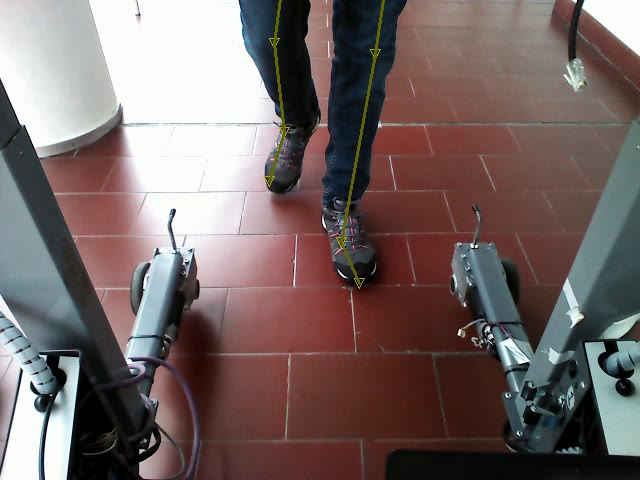
\includegraphics[width=0.98\textwidth]{images/building/results/frameGT10.png}
    \captionof{figure}{Frame 10 Ground Truth}
\end{minipage}%
\begin{minipage}{.5\textwidth}
  \centering
    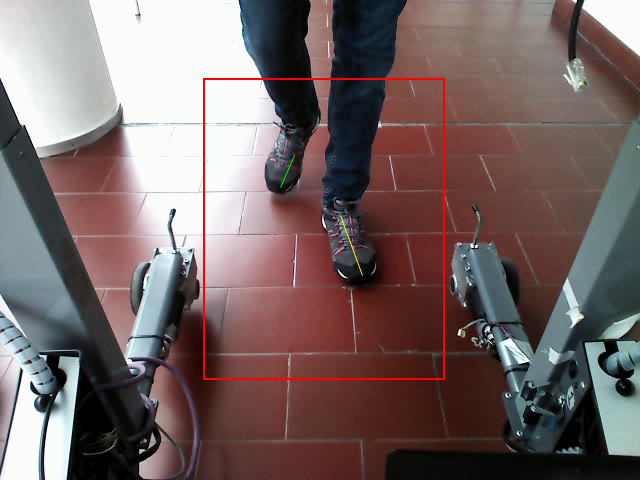
\includegraphics[width=0.98\textwidth]{images/building/results/frame10.png}
    \captionof{figure}{Nosso Frame 10}
    \label{img:Frame10}
\end{minipage}%
\end{figure}

% \begin{figure}[H]
% \centering
% \begin{minipage}{.5\textwidth}
%   \centering
%     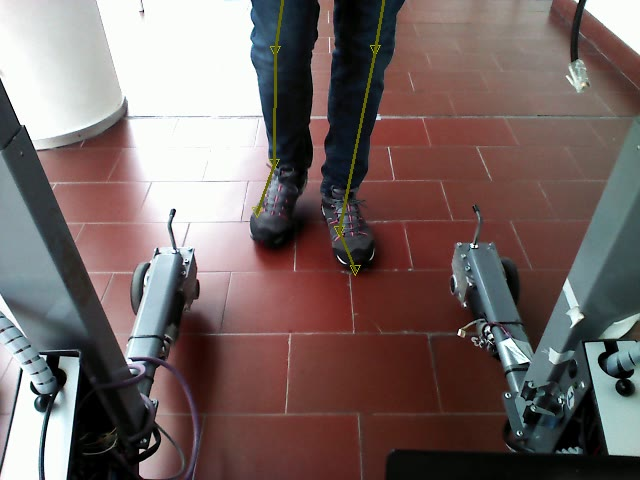
\includegraphics[width=0.98\textwidth]{images/building/results/frameGT15.png}
%     \captionof{figure}{Frame 15 Ground Truth}
% \end{minipage}%
% \begin{minipage}{.5\textwidth}
%   \centering
%     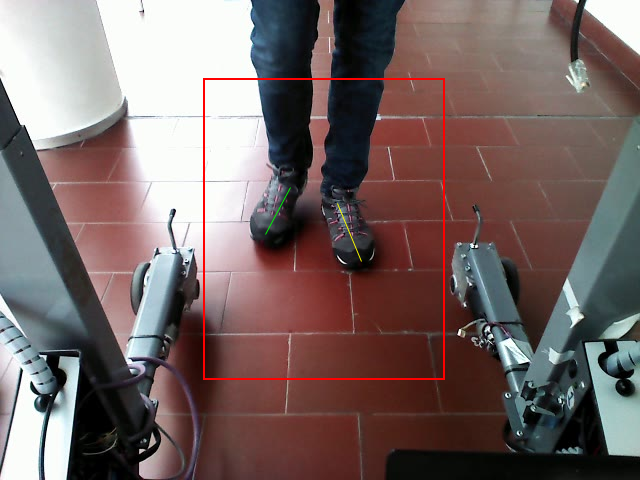
\includegraphics[width=0.98\textwidth]{images/building/results/frame15.png}
%     \captionof{figure}{Nosso Frame 15}
% \end{minipage}%
% \end{figure}

\begin{figure}[H]
\centering
\begin{minipage}{.5\textwidth}
  \centering
    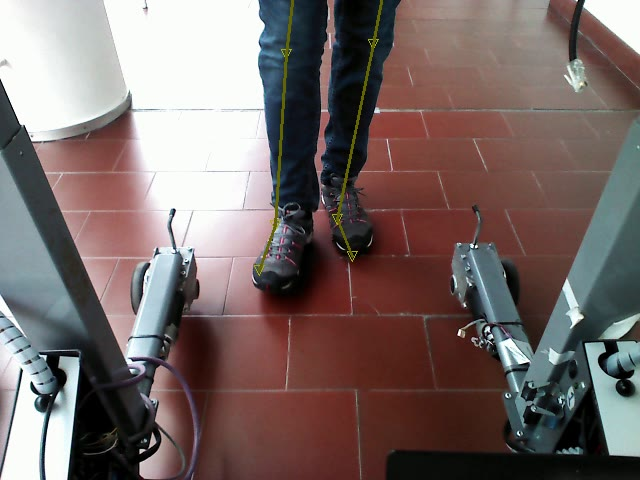
\includegraphics[width=0.98\textwidth]{images/building/results/frameGT20.png}
    \captionof{figure}{Frame 20 Ground Truth}
\end{minipage}%
\begin{minipage}{.5\textwidth}
  \centering
    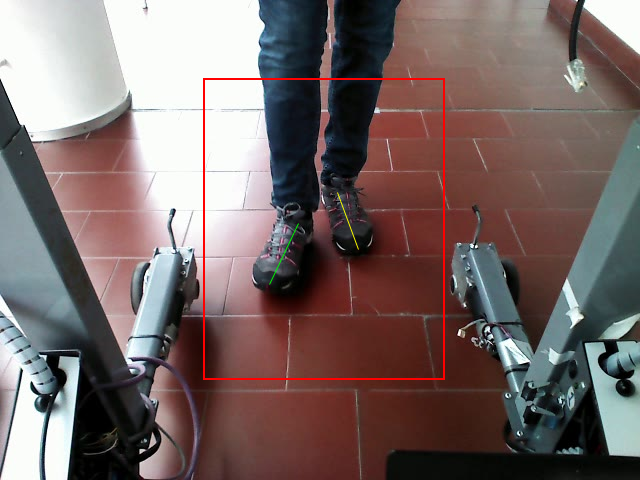
\includegraphics[width=0.98\textwidth]{images/building/results/frame20.png}
    \captionof{figure}{Nosso Frame 20}
    \label{img:Frame20}
\end{minipage}%
\end{figure}

% \begin{figure}[H]
% \centering
% \begin{minipage}{.5\textwidth}
%   \centering
%     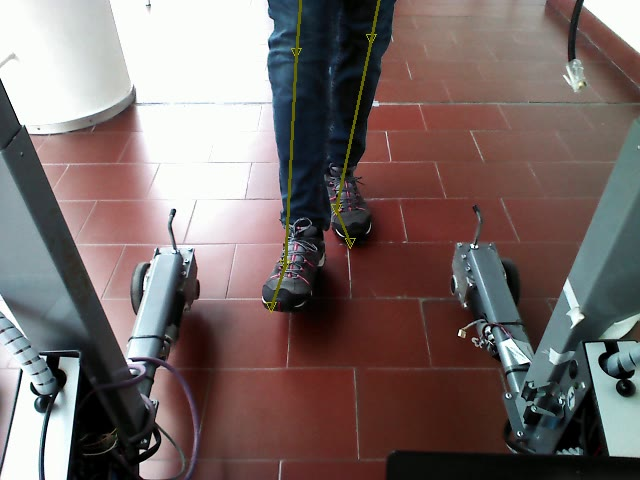
\includegraphics[width=0.98\textwidth]{images/building/results/frameGT25.png}
%     \captionof{figure}{Frame 25 Ground Truth}
% \end{minipage}%
% \begin{minipage}{.5\textwidth}
%   \centering
%     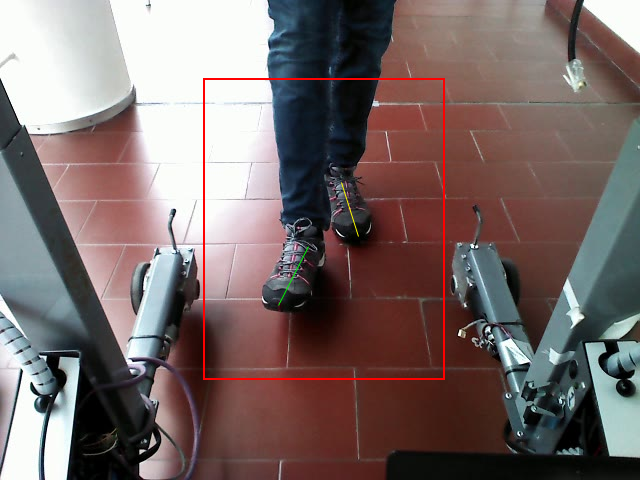
\includegraphics[width=0.98\textwidth]{images/building/results/frame25.png}
%     \captionof{figure}{Nosso Frame 25}
% \end{minipage}%
% \end{figure}

\begin{figure}[H]
\centering
\begin{minipage}{.5\textwidth}
  \centering
    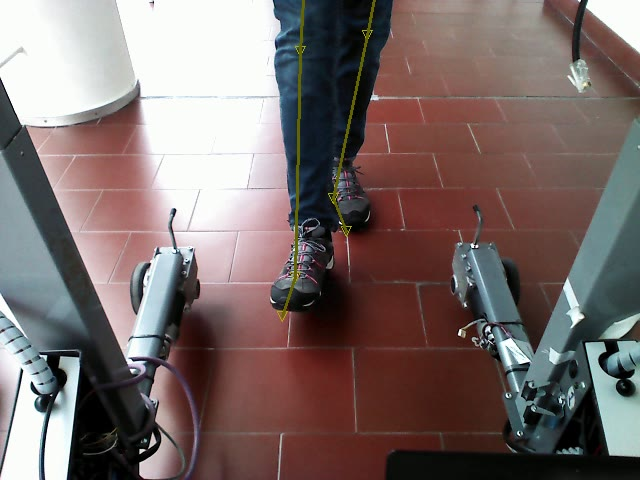
\includegraphics[width=0.98\textwidth]{images/building/results/frameGT30.png}
    \captionof{figure}{Frame 30 Ground Truth}
\end{minipage}%
\begin{minipage}{.5\textwidth}
  \centering
    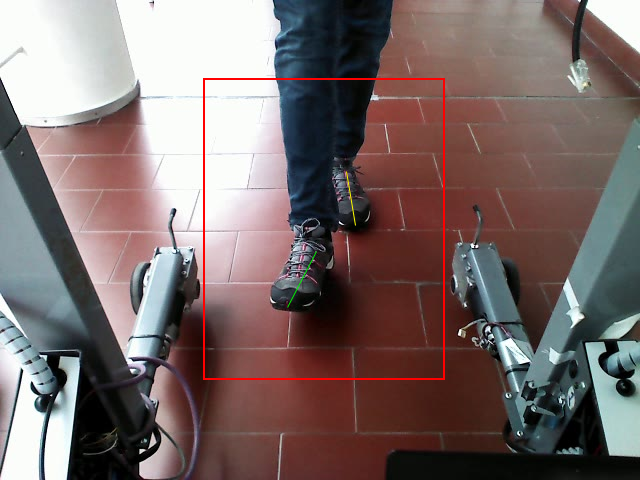
\includegraphics[width=0.98\textwidth]{images/building/results/frame30.png}
    \captionof{figure}{Nosso Frame 30}
    \label{img:Frame30}
\end{minipage}%
\end{figure}

% \begin{figure}[H]
% \centering
% \begin{minipage}{.5\textwidth}
%   \centering
%     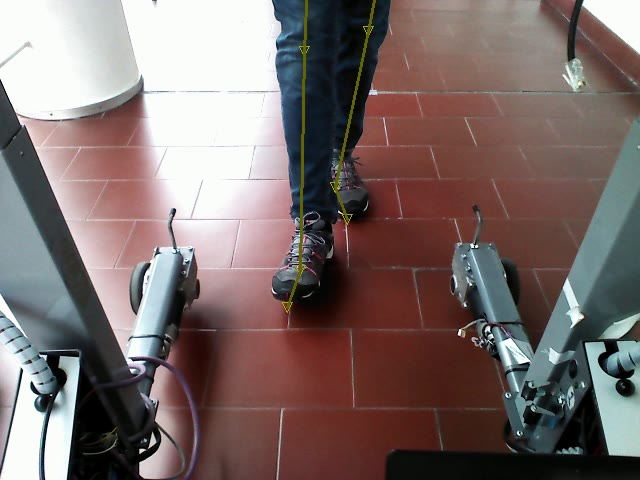
\includegraphics[width=0.98\textwidth]{images/building/results/frameGT35.png}
%     \captionof{figure}{Frame 35 Ground Truth}
% \end{minipage}%
% \begin{minipage}{.5\textwidth}
%   \centering
%     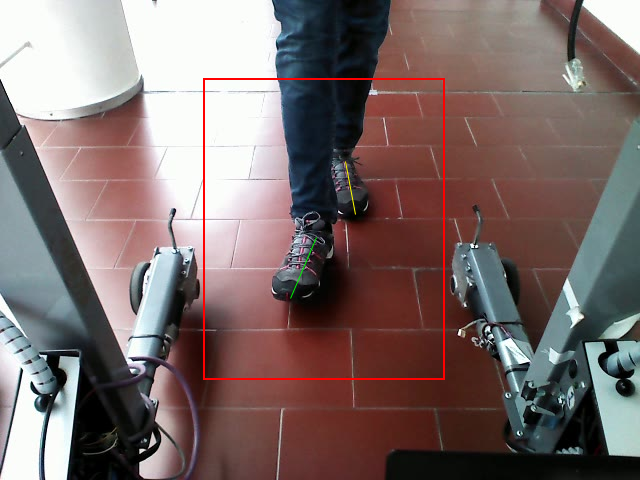
\includegraphics[width=0.98\textwidth]{images/building/results/frame35.png}
%     \captionof{figure}{Nosso Frame 35}
% \end{minipage}%
% \end{figure}

\begin{figure}[H]
\centering
\begin{minipage}{.5\textwidth}
  \centering
    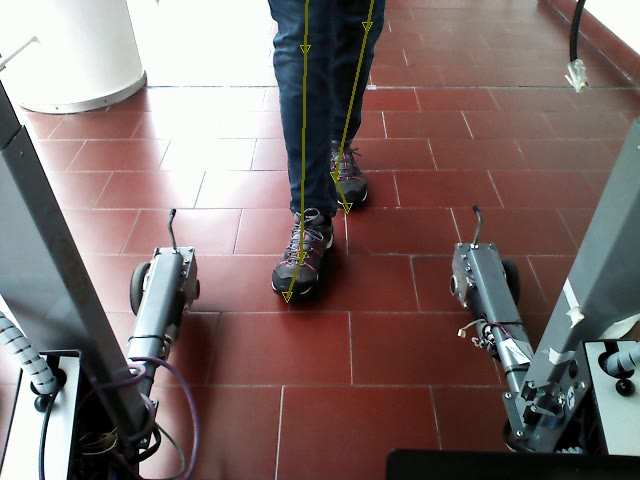
\includegraphics[width=0.98\textwidth]{images/building/results/frameGT40.png}
    \captionof{figure}{Frame 40 Ground Truth}
\end{minipage}%
\begin{minipage}{.5\textwidth}
  \centering
    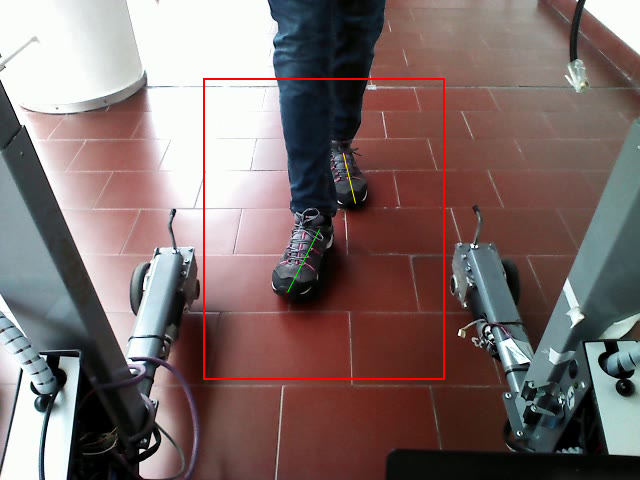
\includegraphics[width=0.98\textwidth]{images/building/results/frame40.png}
    \captionof{figure}{Nosso Frame 40}
    \label{img:Frame40}
\end{minipage}%
\end{figure}

% \begin{figure}[H]
% \centering
% \begin{minipage}{.5\textwidth}
%   \centering
%     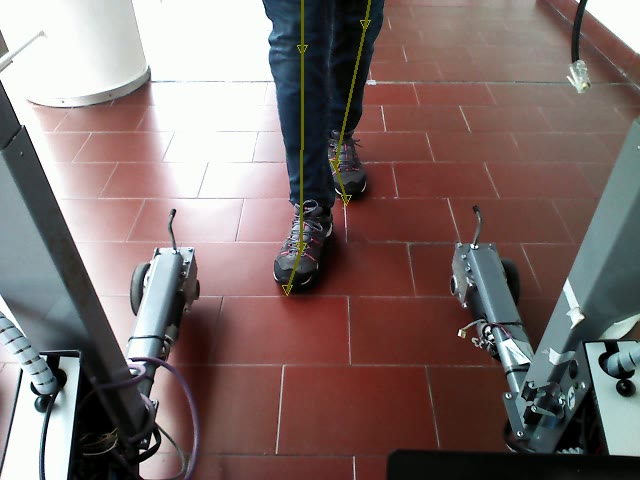
\includegraphics[width=0.98\textwidth]{images/building/results/frameGT45.png}
%     \captionof{figure}{Frame 45 Ground Truth}
% \end{minipage}%
% \begin{minipage}{.5\textwidth}
%   \centering
%     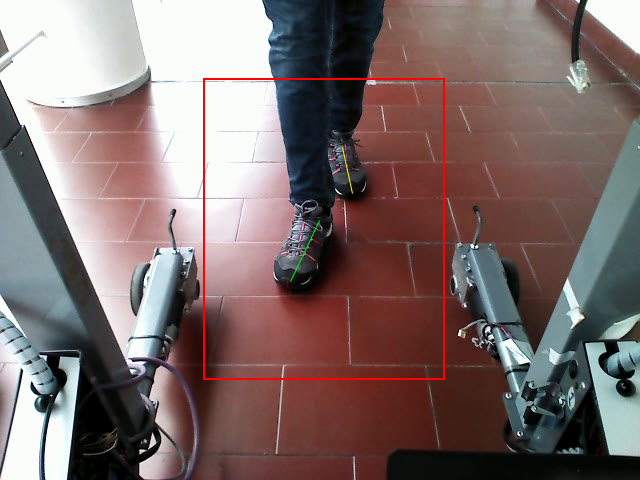
\includegraphics[width=0.98\textwidth]{images/building/results/frame45.png}
%     \captionof{figure}{Nosso Frame 45}
% \end{minipage}%
% \end{figure}

\begin{figure}[H]
\centering
\begin{minipage}{.5\textwidth}
  \centering
    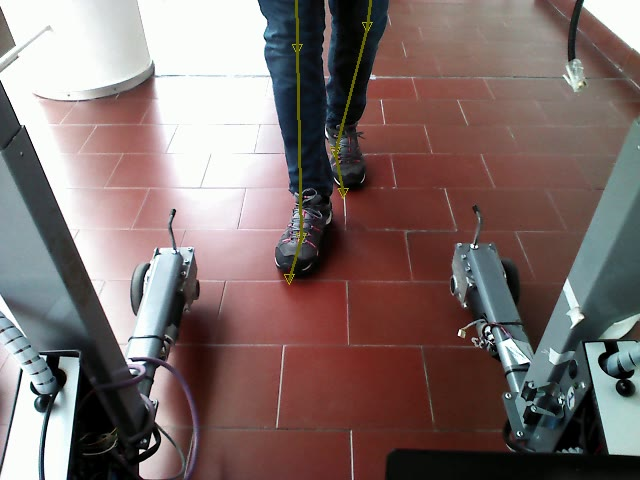
\includegraphics[width=0.98\textwidth]{images/building/results/frameGT50.png}
    \captionof{figure}{Frame 50 Ground Truth}
\end{minipage}%
\begin{minipage}{.5\textwidth}
  \centering
    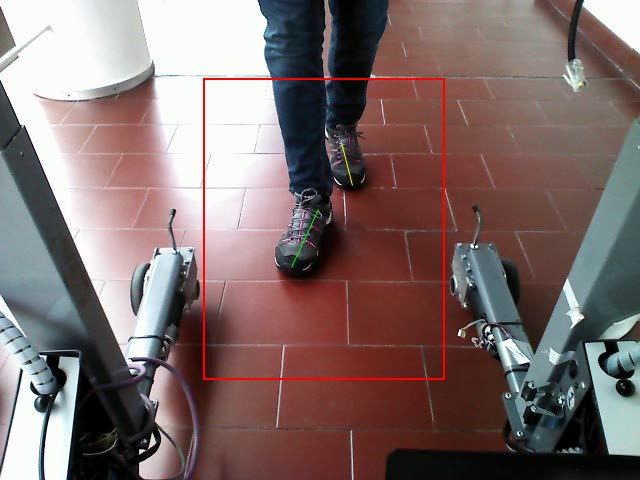
\includegraphics[width=0.98\textwidth]{images/building/results/frame50.png}
    \captionof{figure}{Nosso Frame 50}
    \label{img:Frame50}
\end{minipage}%
\end{figure}

% \begin{figure}[H]
% \centering
% \begin{minipage}{.5\textwidth}
%   \centering
%     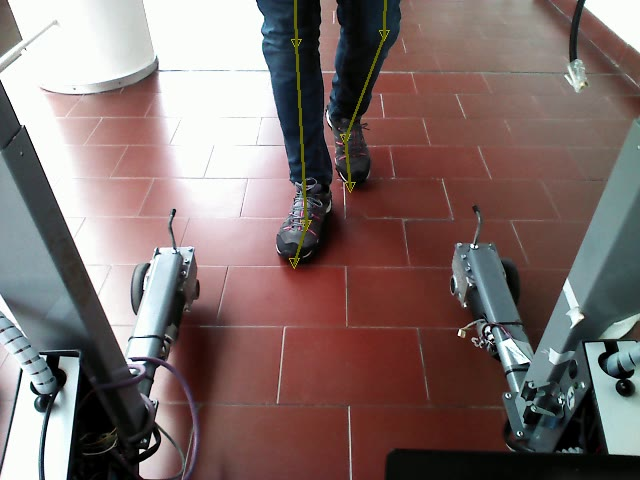
\includegraphics[width=0.98\textwidth]{images/building/results/frameGT55.png}
%     \captionof{figure}{Frame 55 Ground Truth}
% \end{minipage}%
% \begin{minipage}{.5\textwidth}
%   \centering
%     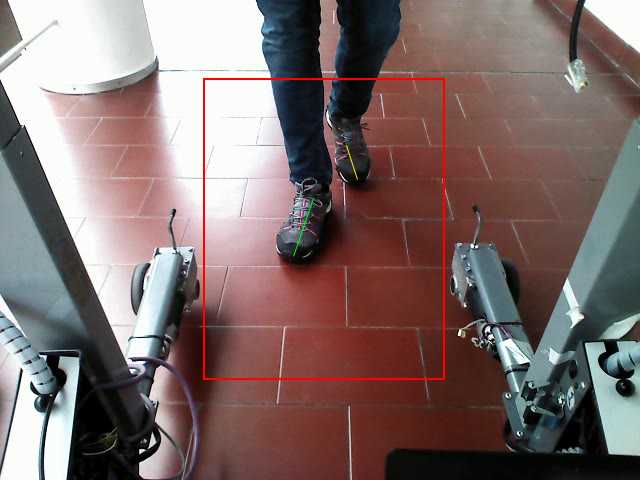
\includegraphics[width=0.98\textwidth]{images/building/results/frame55.png}
%     \captionof{figure}{Nosso Frame 55}
% \end{minipage}%
% \end{figure}

\begin{figure}[H]
\centering
\begin{minipage}{.5\textwidth}
  \centering
    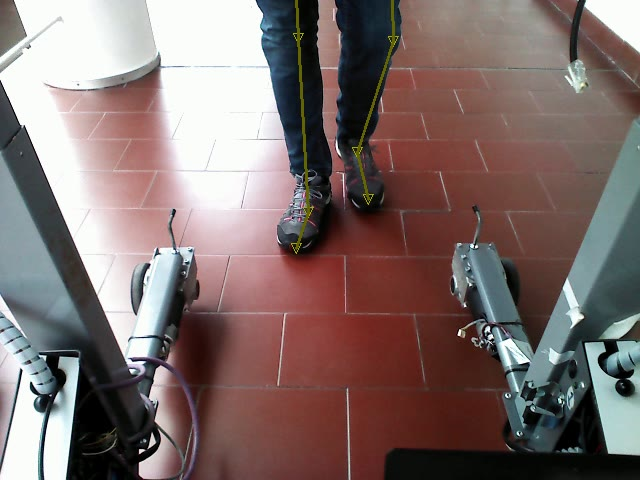
\includegraphics[width=0.98\textwidth]{images/building/results/frameGT59.png}
    \captionof{figure}{Frame 59 Ground Truth}
\end{minipage}%
\begin{minipage}{.5\textwidth}
  \centering
    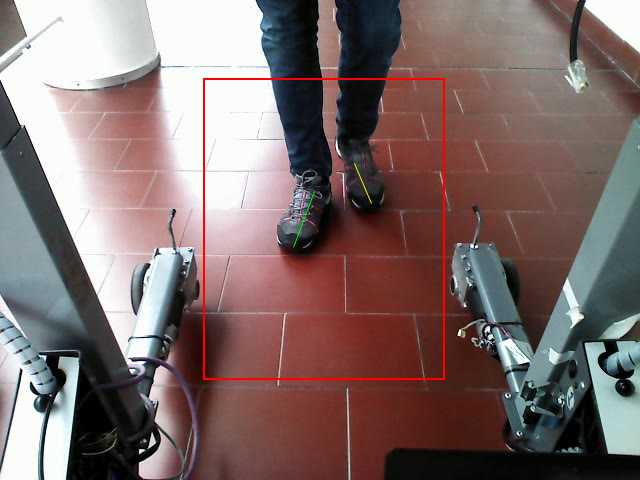
\includegraphics[width=0.98\textwidth]{images/building/results/frame59.png}
    \captionof{figure}{Nosso Frame 59}
    \label{img:Frame59}
\end{minipage}%
\end{figure}


\end{document}